\documentclass[lettersize,journal]{IEEEtran}
\usepackage{amsmath,amsfonts,amssymb}
\usepackage{algorithmic}
\usepackage{algorithm}
\usepackage{array}
\usepackage{tabularx}
\usepackage[caption=false,font=normalsize]{subfig}
\usepackage{textcomp}
\usepackage{stfloats}
\usepackage{url}
\usepackage{verbatim}
\usepackage{graphicx}
\usepackage{cite}
\usepackage{hyperref}
\usepackage{bm}
\usepackage{tikz}
\usetikzlibrary{arrows.meta}
\usepackage{pifont}
\usepackage{amsthm}
\newtheorem{lemma}{Lemma}
\newtheorem{proposition}{Proposition}
\newtheorem{theorem}{Theorem}
\newtheorem{corollary}{Corollary}
\theoremstyle{remark}
\newtheorem{remark}{Remark}
\usepackage{xcolor}
\newcommand{\rev}[1]{\textcolor{blue}{#1}}
\newcommand{\todo}[1]{\textcolor{red}{\textbf{[TODO: #1]}}}   % unfinished parts shown in bold red
\newcommand{\draftnote}[1]{\par\noindent\textcolor{red}{\textbf{$\blacktriangleright$ DRAFT: #1}}\par\medskip}
% placeholder for a not-yet-final figure: \figph{height}{short description}
\newcommand{\figph}[2]{\fcolorbox{red}{gray!8}{\parbox[c][#1][c]{0.96\linewidth}{\centering
\color{red!65!black}\small\textbf{[figure placeholder]}\\[3pt] #2}}}
\graphicspath{{figs/}}
\hyphenation{op-tical net-works semi-conduc-tor IEEE-Xplore Koop-man}

\begin{document}

\title{Bilinear by Default:\\
Koopman Rollouts for Sampling-Based Predictive Control}

% Author intentionally omitted for blind submission.
% \author{Author Name(s)\thanks{Affiliation / funding.}}

\maketitle

\begin{abstract}
The rollout model is the central design choice in sampling-based predictive control: Model Predictive Path Integral (MPPI) control is derivative-free and massively parallel, but only as good as the model through which it rolls out trajectories.
Koopman operator models are attractive here, lifting nonlinear dynamics to an almost-linear evolution whose rollouts are inexpensive matrix--vector products with data-driven error bounds.
Existing Koopman-MPPI keeps the lifted model \emph{linear in the input}, inheriting a restriction that convex Koopman MPC needs but sampling-based control does not.
This paper argues it should simply be dropped: for control-affine systems the provably correct \emph{bilinear} Koopman model is the right default rollout, usable at the same matrix--vector cost precisely because sampling imposes no convexity.
Keeping the lift linear is then not a neutral simplification but a structural forfeiture: it averages the state-dependent input map into a constant, erasing the input channel exactly when the input couples to the tracked motion through a configuration-dependent map such as a vehicle's heading or a manipulator's Jacobian.
An online error-tube cost with a free-energy practical-stability guarantee makes the rollout error-aware, while a first- versus second-order criterion delimits the narrow regime where a linear lift still suffices.
Across MuJoCo benchmarks it parks a nonholonomic vehicle in $95\%$ of trials across seeds, matching a true-dynamics oracle, where linear deep-Koopman MPPI structurally fails ($0\%$); on a manipulator the linear model reaches no target on any seed, whereas the bilinear lift, when its high-dimensional fit converges, reaches them at oracle accuracy, and it needs a four times smaller lifting network where both succeed.
Full hyperparameters and supplementary videos are on the project page: \url{https://koopman_mppi_anonymous.github.io}.
\end{abstract}

\begin{IEEEkeywords}
Model predictive path integral control, Koopman operator, bilinear systems, sampling-based MPC, optimization and optimal control, robot learning.
\end{IEEEkeywords}

%==============================================================
\section{Introduction}\label{sec:intro}
%==============================================================
\IEEEPARstart{S}{ampling-based} model predictive control, most prominently Model Predictive Path Integral (MPPI) control~\cite{williams2016aggressive,williams2017mppi,williams2018mppi}, has become a workhorse for agile robotics.
It is derivative-free, embarrassingly parallel on GPUs, and, through its information-theoretic derivation~\cite{kappen2005,theodorou2010}, places essentially no structural requirement on the dynamics it rolls out.
This generality comes at a price that is easy to overlook: at every control step the controller propagates thousands of sampled trajectories over a horizon, so the \emph{rollout model} is both the dominant computational cost and the single most important design choice.
A high-fidelity physics engine or neural network gives accurate rollouts but is slow; a crude analytical model is fast but biases the control.
The quality of MPPI is, to first order, the quality of this speed--accuracy trade-off~\cite{park2026review}.

The Koopman operator offers a principled way to make the trade favorable.
By lifting the state through a dictionary of observables~\cite{koopman1931,mezic2005,williams2015edmd}, the nonlinear dynamics become (near-)linear in the lifted space, so a rollout reduces to a sequence of matrix--vector products that are orders of magnitude cheaper than integrating the original dynamics, are trivially parallelized, and, where no analytical model is available, identified directly from data~\cite{proctor2016dmdc,lusch2018deep}.
Recent work couples this idea with MPPI and reports substantial speedups using a learned \emph{linear} Koopman model~\cite{mppidk2026}.
Throughout, we assume the analytical dynamics are unknown or too costly to integrate at the sampling rate (the standard model-free, real-time setting), so that a true-dynamics rollout is available only as an \emph{oracle} reference, not as a deployable controller.

\begin{figure}[t]
\centering
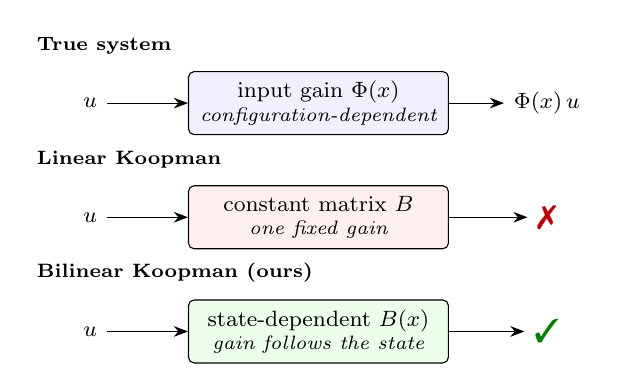
\begin{tikzpicture}[
  >={Stealth[length=1.8mm]}, font=\footnotesize,
  gain/.style={draw, rounded corners=2pt, minimum height=8mm, minimum width=33mm, align=center, inner sep=2pt},
]
\node[gain, fill=blue!6]   (gT) at (0,0)     {input gain $\Phi(x)$\\[-1pt]\scriptsize\itshape configuration-dependent};
\node[gain, fill=red!6]    (gL) at (0,-1.45) {constant matrix $B$\\[-1pt]\scriptsize\itshape one fixed gain};
\node[gain, fill=green!8]  (gB) at (0,-2.9)  {state-dependent $B(x)$\\[-1pt]\scriptsize\itshape gain follows the state};
\node (uT) at (-2.9,0)     {$u$};   \node (uL) at (-2.9,-1.45) {$u$};   \node (uB) at (-2.9,-2.9) {$u$};
\node (oT) at (2.9,0)      {$\Phi(x)\,u$};
\node (oL) at (2.9,-1.45)  {\large\textcolor{red!75!black}{\ding{55}}};
\node (oB) at (2.9,-2.9)   {\large\textcolor{green!50!black}{\ding{51}}};
\draw[->](uT)--(gT); \draw[->](gT)--(oT);
\draw[->](uL)--(gL); \draw[->](gL)--(oL);
\draw[->](uB)--(gB); \draw[->](gB)--(oB);
\node[anchor=south west, font=\scriptsize\bfseries] at (-3.7,0.5)   {True system};
\node[anchor=south west, font=\scriptsize\bfseries] at (-3.7,-0.95) {Linear Koopman};
\node[anchor=south west, font=\scriptsize\bfseries] at (-3.7,-2.4)  {Bilinear Koopman (ours)};
\end{tikzpicture}
\caption{Why the lift must be bilinear. The command $u$ reaches the tracked output through a \emph{configuration-dependent} gain $\Phi(x)$ (a heading rotation $R(\theta)$ for a vehicle, a Jacobian $J(q)$ for an arm), so the input's effect is $\Phi(x)\,u$. A \emph{linear} Koopman lift captures the input-free motion but must apply a single \emph{constant} input matrix, so it cannot reproduce the state-dependent gain (\textcolor{red!75!black}{\ding{55}}). A \emph{bilinear} lift instead lets the input gain $B(x)$ follow the state and matches $\Phi(x)$ (\textcolor{green!50!black}{\ding{51}}), at the same rollout cost; this is made precise in Prop.~\ref{prop:crit}.}
\label{fig:concept}
\end{figure}

The choice of a \emph{linear} lift, however, carries a structural cost that has gone unexamined.
A linear Koopman model lets the input act through a single, fixed map, the same regardless of the robot's configuration.
Yet for a large and important class of robots the input does not act this way.
A wheeled vehicle's speed command moves it along its current heading; a manipulator's joint-velocity command moves the end-effector through its configuration-dependent Jacobian; a legged or whole-body platform drives its task frame through a contact- and posture-dependent map.
The pattern is general: across a broad class of robots the input reaches the tracked output through a \emph{configuration-dependent} gain that no constant input map can reproduce (Fig.~\ref{fig:concept}).
Neither gain is fixed; each rotates or reshapes with the state, so the linear lift simply averages it away.
The \emph{bilinear} Koopman model, the provably correct minimal class for control-affine systems~\cite{iacob2024}, captures precisely this coupling by letting the input multiply the lifted state, and has itself proven effective for control~\cite{bruder2021bilinear,folkestad2021,mamakoukas2019}, but only within model predictive control, where the resulting optimization is no longer convex.
Linear-predictor Koopman MPC keeps the program convex by construction~\cite{korda2018mpc,strasser2026}; sampling-based MPPI carries no such requirement, so the linear restriction is unnecessary.

This is a structural limitation, not a tuning issue: a constant input matrix \emph{must} fail wherever the gain varies with configuration, and we formalize it as Prop.~\ref{prop:crit}.
Because sampling-based control imposes no convexity, we can simply drop the restriction and make the bilinear model the default rollout, at the same matrix--vector regime as the linear one.
We further make the controller model-error-aware by injecting Koopman's proportional error bound~\cite{strasser2026,safedmd2024} as an online error-tube cost (a sampling-based counterpart to robust MPC~\cite{williams2018robust}), and provide a free-energy practical-stability guarantee whose ultimate bound vanishes with the model error.
A first- versus second-order criterion then draws the exact boundary of the claim, marking the narrow second-order regime in which a linear lift remains sufficient; it is a scope tool, not the headline.

\noindent Our contributions are:
\begin{itemize}
\item \textbf{A representational limitation of linear Koopman lifts.} We identify why linear Koopman models fail for a broad class of robots: a constant input matrix cannot encode a configuration-dependent input gain, so on first-order coupling the linear lift forfeits the input channel rather than merely degrading; this is formalized as Prop.~\ref{prop:crit} (Sec.~\ref{sec:method}).
\item \textbf{Bilinear is the right default, at no extra cost.} Because sampling imposes no convexity, the provably correct bilinear class removes this limitation at the same matrix--vector cost as a linear rollout, turning structural failure into success (Sec.~\ref{sec:method},~\ref{sec:exp}).
\item \textbf{Error-aware and stable by construction.} We inject the Koopman proportional error bound as an online error-tube cost and establish a free-energy practical-stability guarantee whose ultimate bound vanishes with the model error (Sec.~\ref{sec:method}).
\item \textbf{The default's boundary, exactly drawn.} A first- versus second-order geometric criterion closes the precise condition under which a linear lift is \emph{exempted}, demoting the linear case from a competing option to a delimited corner (Sec.~\ref{sec:method},~\ref{sec:conclusion}).
\end{itemize}

%==============================================================
\section{Problem Statement and Background}\label{sec:background}
%==============================================================
\textbf{System and objective.}
We consider a control-affine system $\dot x = f(x)+G(x)u$, $x\in\mathbb R^n$, $u\in\mathbb R^m$, discretized as
\begin{equation}\label{eq:dyn}
x_{k+1} = F(x_k,u_k),
\end{equation}
known only through input--state data $\{(x_k,u_k,x_{k+1})\}$.
Over a horizon $T$, the controller seeks the input sequence $U=(u_0,\dots,u_{T-1})$ that minimizes the expected cost
\begin{equation}\label{eq:cost}
J(U) = \mathbb{E}\Big[\phi(x_T) + \textstyle\sum_{k=0}^{T-1} q(x_k,u_k)\Big].
\end{equation}

\textbf{Information-theoretic MPPI.}
MPPI draws $K$ input sequences $V^{(k)}=U+\mathcal{E}^{(k)}$ with $\varepsilon_t^{(k)}\sim\mathcal N(0,\Sigma)$, rolls each through the dynamics to obtain a trajectory cost $S(V^{(k)})$, and updates each input by the cost-weighted average of the sampled perturbations,
\begin{equation}\label{eq:mppi}
\begin{aligned}
u_t &\leftarrow u_t + \frac{\sum_{k} w^{(k)}\,\varepsilon_t^{(k)}}{\sum_k w^{(k)}},\\[2pt]
w^{(k)} &= \exp\!\Big(-\tfrac1\lambda\big(S(V^{(k)})-\rho\big)\Big),
\end{aligned}
\end{equation}
with temperature $\lambda>0$ and $\rho=\min_k S(V^{(k)})$.
The information-theoretic derivation places no convexity, differentiability, or affine-in-input requirement on $F$~\cite{williams2018mppi}; the only step that scales with the sample count is the per-sample \emph{rollout} used to evaluate $S(V^{(k)})$.

\textbf{Koopman lifting and identification.}
Koopman methods lift the state through a dictionary $\Psi:\mathbb R^n\to\mathbb R^N$ with $\Psi(0)=0$ and a left inverse $C$ (so $x=C\,\Psi(x)$), and model the evolution of the lifted state $z=\Psi(x)$.
The \emph{linear} and \emph{bilinear} predictors are
\begin{align}
\text{(linear)}\quad & z^+ \approx A z + B u, \label{eq:lin}\\
\text{(bilinear)}\quad & z^+ \approx A z + B_0 u + \textstyle\sum_{i=1}^m u_i\,(B_i z). \label{eq:bil}
\end{align}
Because the input enters the lifted dynamics through state-dependent vector fields, a finite \emph{linear} predictor is generically inexact, whereas the \emph{bilinear} form~\eqref{eq:bil} is the provably correct minimal class~\cite{iacob2024}.
Both are identified by (regularized) least squares, using extended dynamic mode decomposition with control~\cite{williams2015edmd,proctor2016dmdc} for a fixed dictionary or jointly with a learned deep dictionary~\cite{lusch2018deep}, so that \eqref{eq:bil} simply augments the regressor with the products $u_i z$.
Writing $M(u):=A+\sum_i u_i B_i$, one bilinear step is $z^+=M(u)z+B_0u$: an input-dependent matrix, but still $m{+}1$ matrix--vector products, the same rollout regime as the linear model~\eqref{eq:lin}.

\textbf{Proportional error bound.}
Let $r(x,u)$ be the one-step residual of~\eqref{eq:bil}.
Certified Koopman identification~\cite{strasser2026,safedmd2024} provides a \emph{proportional} error bound
\begin{equation}\label{eq:propbound}
\|r(x,u)\| \;\le\; c_x\,\|\Psi(x)\| + c_u\,\|u\|,
\end{equation}
whose constants $c_x,c_u$ are estimated from data and \emph{vanish at the equilibrium}.
This bound underlies the closed-loop guarantees of Koopman control; in Sec.~\ref{sec:method} we propagate it into the sampling cost.

%==============================================================
\section{Method: Bilinear Koopman MPPI}\label{sec:method}
%==============================================================
Our controller is standard information-theoretic MPPI~\eqref{eq:mppi}, but every rollout is performed in the lifted space by the \emph{bilinear} surrogate~\eqref{eq:bil}.
At each control step we lift the measured state, roll $K$ sampled input sequences through $\hat z^+ = M(v)\hat z + B_0 v$, score them with the task cost plus an error-tube penalty, and apply the softmax-weighted update (Algorithm~\ref{alg:kmppi}).
Each rollout step is one $N\times N$ product for $A$, $m$ for the $\{B_i\}$, and the affine term $B_0u$---an $m{+}1$ factor over the single product of a linear model~\eqref{eq:lin}.
For the small input dimensions typical in robotics this is a modest constant, and the $K$ samples and $m$ products fuse into dense batched matrix multiplications on a GPU, so the wall-clock cost is set by the lifted dimension $N$, not by the bilinear structure.

\begin{algorithm}[t]
\caption{Bilinear Koopman MPPI (one control step)}\label{alg:kmppi}
\begin{algorithmic}[1]
\REQUIRE state $x$; warm start $U$; model $A,B_0,\{B_i\}_{i=1}^m,C$; bound $c_x,c_u$; weights $\lambda,\beta$
\STATE $z_0 \leftarrow \Psi(x)$
\FOR{$k=1,\dots,K$ \textbf{in parallel}}
  \STATE $V^{(k)} \leftarrow U + \mathcal E^{(k)}$, \quad $\varepsilon_t^{(k)}\sim\mathcal N(0,\Sigma)$
  \STATE $\hat z \leftarrow z_0$,\; $e\leftarrow 0$,\; $S^{(k)}\leftarrow 0$
  \FOR{$t=0,\dots,T-1$}
    \STATE $\hat z \leftarrow M(v_t^{(k)})\,\hat z + B_0\,v_t^{(k)}$
    \STATE $e \leftarrow \big(\|M(v_t^{(k)})\|+c_x\big)e + c_x\|\hat z\| + c_u\|v_t^{(k)}\|$
    \STATE $S^{(k)} \leftarrow S^{(k)} + q\big(C\hat z, v_t^{(k)}\big) + \beta\, e$
  \ENDFOR
  \STATE $S^{(k)} \leftarrow S^{(k)} + \phi(C\hat z)$
\ENDFOR
\STATE $w^{(k)} \leftarrow \exp\!\big(-\tfrac1\lambda(S^{(k)}-\min_j S^{(j)})\big)$
\STATE $U \leftarrow U + \big(\textstyle\sum_k w^{(k)}\mathcal E^{(k)}\big)\big/\textstyle\sum_k w^{(k)}$
\STATE \textbf{return} $u_0$;\; shift $U$ for the next step
\end{algorithmic}
\end{algorithm}

\textbf{Training.}
Identifying~\eqref{eq:bil} by one-step regression yields poor multi-step rollouts; we instead minimize a \emph{multi-step} loss over length-$H$ windows,
\begin{equation}\label{eq:trainloss}
\mathcal L = \sum_{t=1}^{H}\big\|C(\hat z_t - z_t)\big\|^2 + \gamma\,\big\|\hat z_t - \Psi(x_t)\big\|^2,
\end{equation}
where $\hat z_t$ is rolled from $\hat z_0=\Psi(x_0)$ through~\eqref{eq:bil} and the second term enforces latent consistency.
Two choices matter in practice: we initialize the bilinear matrices $B_i$ to zero, so training starts from the linear model~\eqref{eq:lin} and can only improve on it; and we draw coherent control sequences that match the deployment distribution rather than white noise.

\textbf{Why bilinear is the right default.}
The bilinear term is what preserves the input channel a linear lift discards, and how much that matters is set by how the input enters the quantity the controller tracks.
Let $y=h(x)=Cz$ be that output.
To first order in the step, the control-affine dynamics give
\begin{equation}\label{eq:firstorder}
\begin{aligned}
y_{k+1}-y_k = {}&\underbrace{\nabla h(x_k)\,f(x_k)\,\Delta t}_{d(x_k)}\\[2pt]
&+ \underbrace{\nabla h(x_k)\,G(x_k)\,\Delta t}_{\Phi(x_k)}\,u_k + O(\Delta t^2),
\end{aligned}
\end{equation}
so the input enters $y$ through the state-dependent gain $\Phi(x)$.

\begin{proposition}[A constant input matrix cannot encode a state-dependent gain]\label{prop:crit}
Let the tracked output $y=Cz$ evolve, to first order in the step, as $y_{k+1}=y_k+\Phi(x_k)\,u_k+d(x_k)$ with input gain $\Phi(x)$.
A linear Koopman model~\eqref{eq:lin} reproduces this input response for all $(x,u)$ only if $\Phi$ is constant; if $\Phi$ varies with the configuration, the linear model's output error is of the order of the variation of $\Phi$ over the operating set, whereas the bilinear model~\eqref{eq:bil} reproduces $\Phi(x)u$ exactly whenever the dictionary spans the entries of $\Phi$.
\end{proposition}
\noindent\emph{Proof.}
For~\eqref{eq:lin}, $\partial y_{k+1}/\partial u = CB$ is constant, so matching $\Phi(x)$ for all $x$ forces $\Phi\equiv CB$.
For~\eqref{eq:bil}, $\partial y_{k+1}/\partial u_i = C\,(B_0 e_i + B_i z)$ is affine in the lifted state, so $\Phi(x)u$ is reproduced once each entry of $\Phi(x)$ lies in $\mathrm{span}\,\Psi$. \hfill$\square$

\begin{remark}[first- vs.\ second-order coupling]\label{rem:order}
The criterion uses the \emph{first-order} (kinematic) increment of $y$.
A wheeled vehicle (output $y$ the position, gain $\Phi(x)$ the heading rotation) and a manipulator (output the end-effector, gain the Jacobian $J(q)$) fall here, so linear Koopman must fail.
When the input acts at \emph{second} order, through acceleration (a quadrotor's thrust), $\Phi(x)u$ reaches $y$ only after a further integration, the constant-matrix error is $O(\Delta t^2)$ smaller, and a linear lift is not merely sufficient but preferable.
The first-order side is tested in Sec.~\ref{sec:exp}; the second-order side, where the linear default is safe, in Sec.~\ref{sec:conclusion}.
\end{remark}

\emph{Examples.}
For a unicycle (output the planar position) $\Phi(x)\!\propto\!(\cos\theta,\sin\theta)$ rotates with the heading; for a manipulator (output the end-effector, joint-velocity input) $\Phi(q)=J(q)\,\Delta t$ is the Jacobian.
A lift spanning these entries reproduces $\Phi$ exactly, whereas a constant matrix is correct at one configuration only; as $\Phi$ sweeps a wide range its best constant surrogate sits near the average (near zero for the circle-covering unicycle), so the linear model fails outright.

\textbf{Error-tube cost.}
The surrogate is inexact, so we discount samples whose \emph{certified} error is large.
Propagating the proportional bound~\eqref{eq:propbound} along a rollout gives the scalar tube of Algorithm~\ref{alg:kmppi} (line~7), with $e_0=0$,
\begin{equation}\label{eq:tube}
e_{t+1} = \big(\|M(v_t)\|+c_x\big)\,e_t + c_x\|\hat z_t\| + c_u\|v_t\|,
\end{equation}
and we add $\beta\sum_t e_t$ to each sample cost.
Because~\eqref{eq:propbound} vanishes at the equilibrium, this penalty regularizes the search toward the certified region; $\beta\to0$ recovers plain bilinear MPPI, and replacing the expectation by a conditional value-at-risk yields a risk-averse variant.

\begin{proposition}[Tube bound]\label{prop:tube}
Along any shared input sequence, the tube~\eqref{eq:tube} satisfies $\|z_t-\hat z_t\|\le e_t$ for all $t$, and hence $\|x_t-\hat x_t\|\le\|C\|\,e_t$.
\end{proposition}
\noindent\emph{Proof.}
By induction: $e_0=0$ matches $z_0=\hat z_0$.
Assuming $\|z_t-\hat z_t\|\le e_t$, subtract the true and nominal updates, take norms, and bound the residual by~\eqref{eq:propbound} using $\|z_t\|\le\|\hat z_t\|+e_t$; all coefficients are nonnegative, so the bound propagates to $t{+}1$. \hfill$\square$

\textbf{Stability.}
Let $\mathcal F_\bullet(x)=-\lambda\log\mathbb E_{V\sim p}[\exp(-S_\bullet(V;x)/\lambda)]$ be the free energy of the real ($\bullet{=}\mathrm{real}$) and surrogate ($\bullet{=}\mathrm{nom}$) costs.
\begin{theorem}[Free-energy practical stability]\label{thm:stab}
If the surrogate is cost-controllable and the tracked cost is Lipschitz, then the model-induced free-energy gap obeys $|\mathcal F_{\mathrm{real}}-\mathcal F_{\mathrm{nom}}|\le\Delta S_{\max}$, the tube cost of Prop.~\ref{prop:tube}; consequently the real closed loop is practically asymptotically stable with ultimate bound $R=O(c_x,c_u,\lambda,K^{-1/2})$, which vanishes as the model and sampling errors vanish.
\end{theorem}
\noindent\emph{Proof sketch.}
The gap bound follows from $|S_{\mathrm{real}}-S_{\mathrm{nom}}|\le\Delta S_{\max}$ (Prop.~\ref{prop:tube} and cost-Lipschitzness) and monotonicity of $\log\sum\exp$; combined with the relaxed-dynamic-programming decrease of the surrogate value~\cite{strasser2026,korda2018mpc} it gives the ultimate bound.
Only cost-Lipschitzness is needed, not smoothness of the value function.
The full proof and a weighted-norm refinement of~\eqref{eq:tube} (which requires SafEDMD-grade $c_x$) are in the extended version. \hfill$\square$

%==============================================================
\section{Experiments}\label{sec:exp}
%==============================================================
\textbf{Setup.}
The three controllers share a deep Koopman lifting (identical network width, training data, and multi-step loss) and differ only in the lifted model: \emph{Ours} uses the bilinear form~\eqref{eq:bil} and \emph{MPPI-DK}~\cite{mppidk2026} the linear form~\eqref{eq:lin}.
For a fair comparison the two learned controllers share the horizon, sample count, lifting dimension, and training budget of Table~\ref{tab:hp}; where a setting is method-specific we adopt MPPI-DK's own reported choice (for instance the pendulum dictionary width), so the reported gaps reflect the model class rather than baseline under-tuning.
\emph{Oracle} MPPI, rolling out the true dynamics, is a model-fidelity reference, not a performance ceiling: sampling-based MPPI is suboptimal even with the true model.
All systems are simulated in MuJoCo~\cite{mujoco2012}.
Key hyperparameters are listed in Table~\ref{tab:hp}; full settings and the experiment videos are on the project page: \url{https://koopman_mppi_anonymous.github.io}.

\begin{table}[t]\centering
\caption{Key per-system hyperparameters.}\label{tab:hp}
\begin{tabularx}{\linewidth}{l *{5}{>{\centering\arraybackslash}X}}
\hline
System & $N$ & $K$ & $T$ & $\Delta t$ & $\lambda$\\
\hline
Unicycle  & $8$  & $2048$ & $40$ & $0.05$ & $0.5$\\
7-DOF arm & $20$ & $800$  & $15$ & $0.05$ & $0.4$\\
Pendulum  & $11$ & $1536$ & $50$ & $0.05$ & $0.8$\\
Quadrotor & $24$ & $1200$ & $20$ & $0.02$ & $0.6$\\
\hline
\end{tabularx}
\par\smallskip
{\footnotesize $N$, lifted dimension; $K$, samples; $T$, horizon; $\Delta t$, step size; $\lambda$, temperature.}
\end{table}

\subsection{First-order coupling: where linearizing forfeits the input channel}

\begin{figure*}[t]\centering
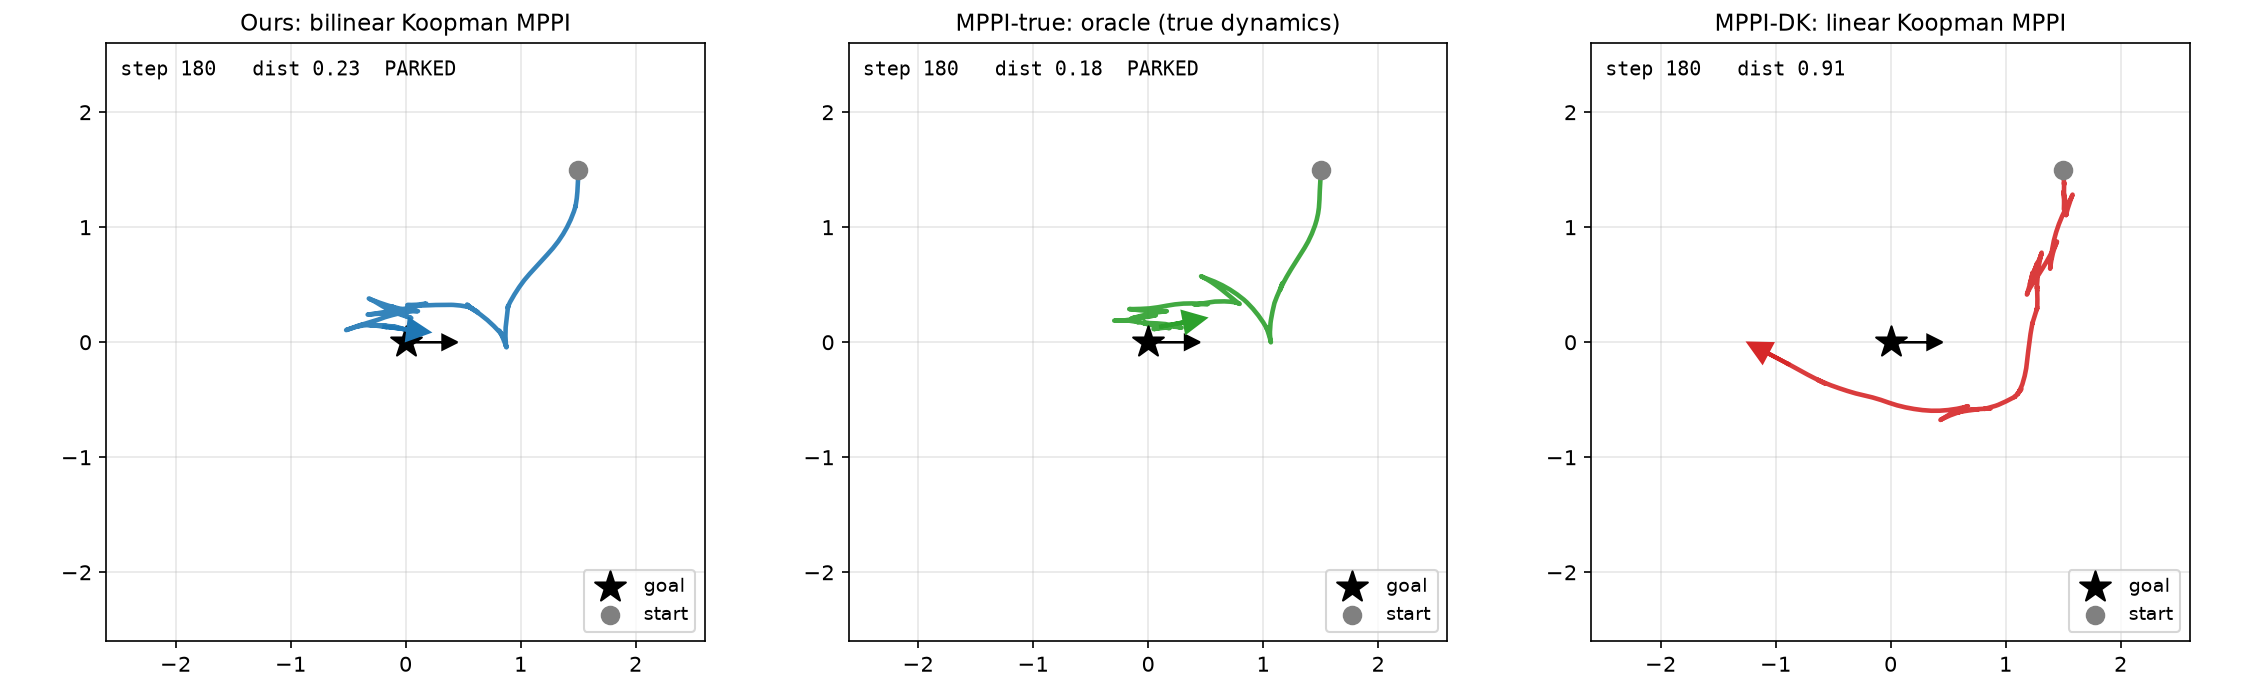
\includegraphics[width=\linewidth]{fig_unicycle.png}
\caption{Nonholonomic unicycle parking (start $\bullet$, goal $\star$; deep Koopman, representative run). Ours (bilinear, left) reaches the goal pose, matching the true-dynamics oracle (centre); MPPI-DK (linear, right) drives off and never converges, since a constant input matrix cannot represent the heading-dependent coupling $v(\cos\theta,\sin\theta)$ (parking rates over $20$ trials: $95/85/0\%$, Sec.~\ref{sec:exp}).}
\label{fig:unicycle}
\end{figure*}

\begin{figure*}[t]\centering
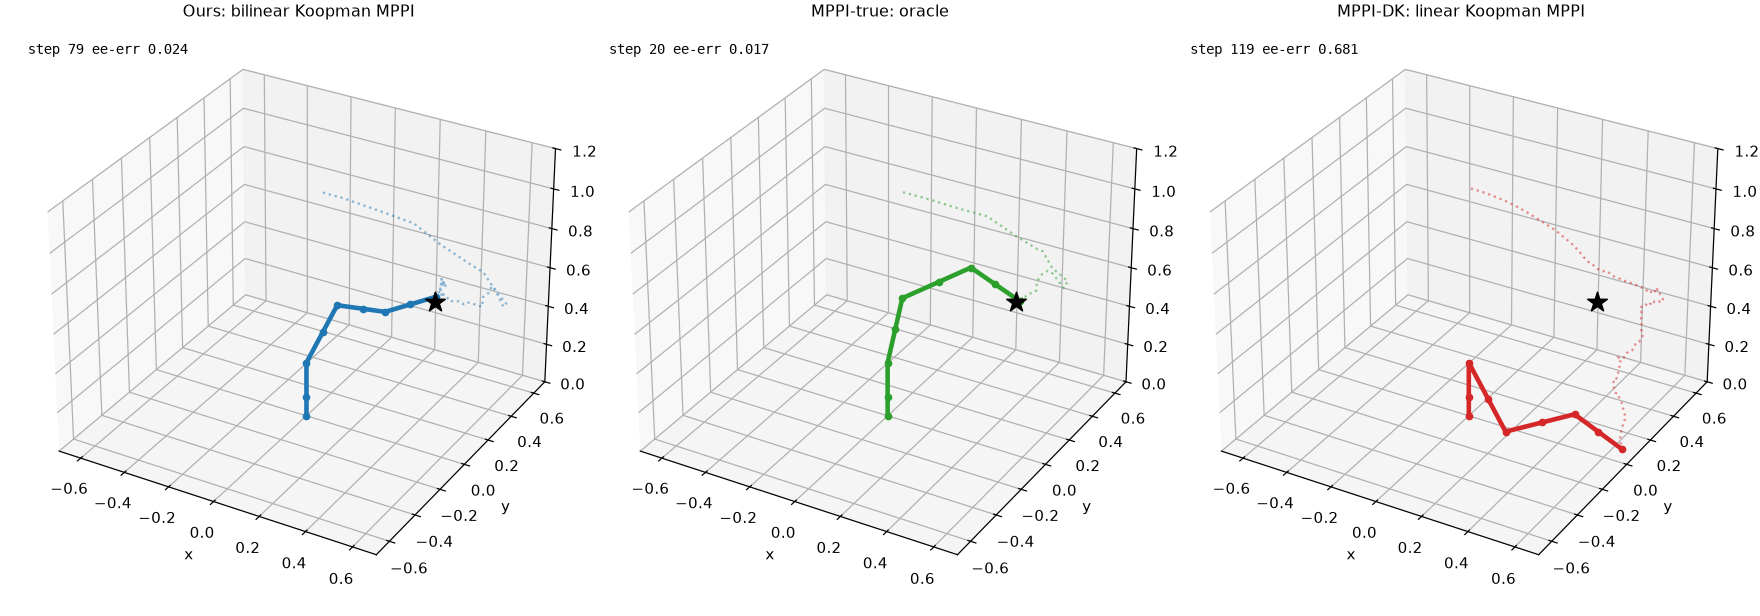
\includegraphics[width=\linewidth]{fig_arm.png}
\caption{7-DOF manipulator end-effector reach (goal $\star$). Ours (bilinear, left) and the oracle (centre) reach the target; MPPI-DK (linear, right) stalls far away, as a constant input matrix cannot represent the configuration-dependent Jacobian $J(q)$.}
\label{fig:arm}
\end{figure*}

\textbf{Nonholonomic vehicle.}
A unicycle must park its pose $(x,y,\theta)$ at a goal; the forward-speed input enters the position through the heading, a configuration-dependent rotation (Prop.~\ref{prop:crit}).
Because the heading sweeps the full circle along a trajectory, the best constant surrogate for the input gain $(\cos\theta,\sin\theta)$ sits near its average, which is essentially zero, so the linear lift retains almost no usable input channel.
The consequence is stark in open loop: rolled out over the horizon, the bilinear model predicts the position $37$--$48\times$ more accurately than the linear one.
In closed loop (Fig.~\ref{fig:unicycle}), ours parks reliably: across five training seeds and four start--goal pairs ($20$ trials), it reaches the goal pose in $95\%$ of trials, matching the true-dynamics oracle ($85\%$), whereas MPPI-DK parks in $0\%$, driving off along its initial heading and ending $3.0\pm1.9$\,m away.

\textbf{7-DOF manipulator.}
A redundant arm must drive its end-effector to a Cartesian target under joint-velocity commands, which enter the end-effector through the configuration-dependent Jacobian $J(q)$.
Over seven Cartesian targets and five training seeds (Figs.~\ref{fig:arm} and~\ref{fig:armbar}), the linear model reaches \emph{none} on any seed, ending $0.62\pm0.26$\,m from the target: the structural failure of Prop.~\ref{prop:crit} once more.
The bilinear model is about five times closer (mean final error $0.13$\,m) and lands at oracle accuracy ($0.03$\,m) on the targets it solves.
Reliability is lower than on the unicycle, however, for an understood reason: the bilinear model carries one input matrix per channel, so the $m{=}7$ lift is harder to optimize and more initialization-sensitive---the mechanism behind our zero-initialization and the naive bilinear quadrotor's instability (Sec.~\ref{subsec:ablation}).
The per-seed reach count thus varies (mean $\sim\!3/7$, best $6/7$), though the linear model never reaches at all, and reliable optimization of the high-DOF bilinear lift is left open (Sec.~\ref{sec:conclusion}).
The open-loop prediction gap is itself modest---about $1.5\times$ on the end-effector (Fig.~\ref{fig:armpred}), since $J(q)$ has a non-zero linearizable mean unlike the sign-flipping unicycle gain---so the win is one of structural representability amplified by control, not of prediction-ratio magnitude.

\begin{figure}[t]\centering
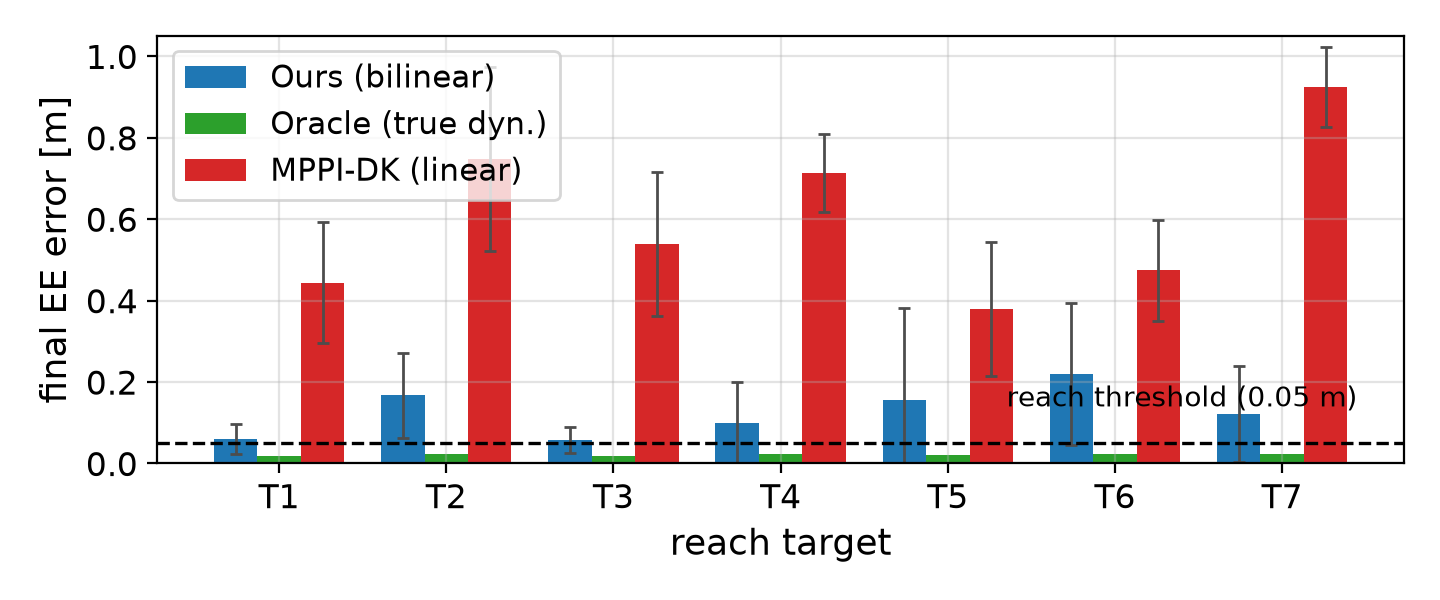
\includegraphics[width=\linewidth]{fig_arm_bar.png}
\caption{Final end-effector error over seven targets (mean $\pm$ s.d.\ across five training seeds). The bilinear model and the oracle stay several times closer to every target than the linear model; MPPI-DK (linear) reaches none on any seed, while the bilinear model lands at oracle accuracy on the targets it solves, with seed-dependent reliability.}
\label{fig:armbar}
\end{figure}

\begin{figure}[t]\centering
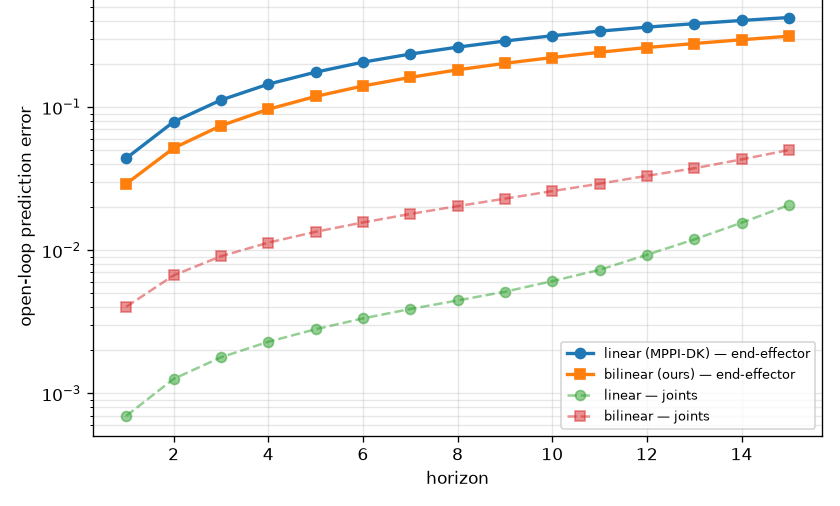
\includegraphics[width=\linewidth]{fig_arm_pred.png}
\caption{7-DOF arm open-loop prediction error vs.\ horizon. On the end-effector the bilinear edge is modest ($\approx1.5\times$), because the Jacobian $J(q)$ has a non-zero linearizable mean; receding-horizon control nonetheless amplifies this structural deficit into the closed-loop gap of Fig.~\ref{fig:armbar}.}
\label{fig:armpred}
\end{figure}

\subsection{Efficiency even where both succeed}
On torque-limited pendulum swing-up the input couples to the tracked angle only weakly, and, consistent with MPPI-DK, all three controllers swing up and balance.
The informative axis here is not success but model capacity.
Fixing the lifted dimension and sweeping the width of the deep dictionary (Fig.~\ref{fig:pendulum}), the bilinear model reaches a given multi-step accuracy with about $4\times$ fewer neurons: ours at $32$ neurons matches the linear model at $128$, and the linear model saturates near a prediction error of $0.50$ without ever reaching the accuracy ($0.26$) that ours attains at the $256$ neurons MPPI-DK report using.
Here bilinearity buys \emph{efficiency} rather than feasibility---the same expressiveness at a fraction of the parameters.

\begin{figure}[t]\centering
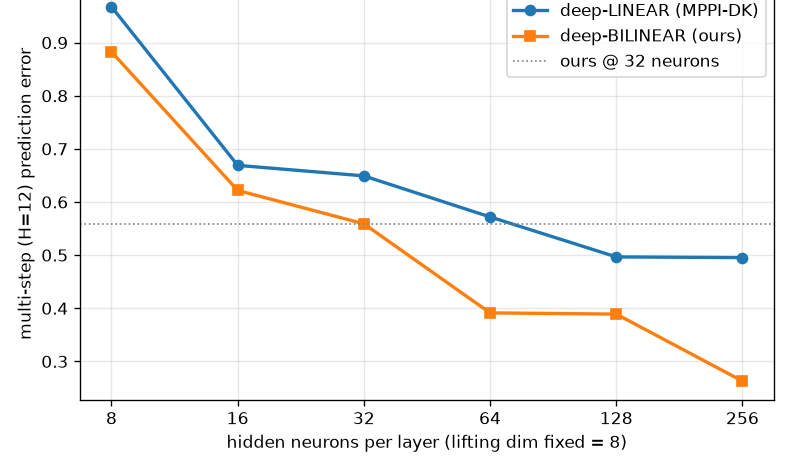
\includegraphics[width=\linewidth]{fig_pendulum_neurons.png}
\caption{Pendulum: multi-step ($H{=}12$) open-loop prediction error vs.\ dictionary width, at fixed lifted dimension. The bilinear model (ours) reaches a target accuracy with $\approx4\times$ fewer neurons; the linear model (MPPI-DK) saturates and never reaches the bilinear accuracy. Both controllers swing up.}\label{fig:pendulum}
\end{figure}

\subsection{Error tube and rollout timing}
\textbf{Tube validity, and the certified-bound caveat.}
Theorem~\ref{thm:stab} and the error tube stand on \emph{certified} constants $c_x,c_u$, which the deep dictionaries used here do not yet supply; we therefore fit the constants by least squares on the deep model's one-step residuals and treat them as an empirical proxy for the certified bound.
Under this proxy the tube is sound: propagated along held-out rollouts of the \emph{deep bilinear} unicycle model, it contains the true lifted error at every step with zero violations over $82{,}000$ rollout steps (Fig.~\ref{fig:tube}), the only out-of-sample violations occurring once a trajectory leaves the region where the bound was fit~\eqref{eq:propbound}.
It is, however, conservative: plain least squares yields $\|A\|_2\!\approx\!1.02$ and $c_x\!\approx\!3.5\times10^{-3}$, so the Euclidean tube compounds to $\sim\!10^{3}\times$ the true error over a $40$-step horizon---valid as a certificate of containment, but loose as a bound.
The looseness is structural rather than a tuning artefact: the kinematic lift is an integrator ($\|A\|_2\!\approx\!1$), so even with the small $c_x$ above, a contractive tube (and with it the ultimate bound of Theorem~\ref{thm:stab}) would require a Schur-stable lifted model that plain least squares does not provide, and forcing stability by eigenvalue clipping inflates $c_x$ back in proportion to the clipping margin.
Certified, stability-constrained identification~\cite{strasser2026,safedmd2024} is therefore the principal next step (Sec.~\ref{sec:conclusion}).

\textbf{Rollout timing.}
The lifted rollout is also why a learned model is preferable to the true-dynamics oracle even in simulation.
For $K{=}1024$ samples over a horizon of $T{=}30$, one bilinear-Koopman rollout costs $3.5$\,ms per control step, against $11$\,ms for a hand-batched integration of the true dynamics ($3\times$) and $72$\,ms for a physics-engine rollout ($20\times$): the same control rate at a fraction of the compute, the $m{+}1$ matrix--vector factor over a linear model being negligible against this gap.

\begin{figure}[t]\centering
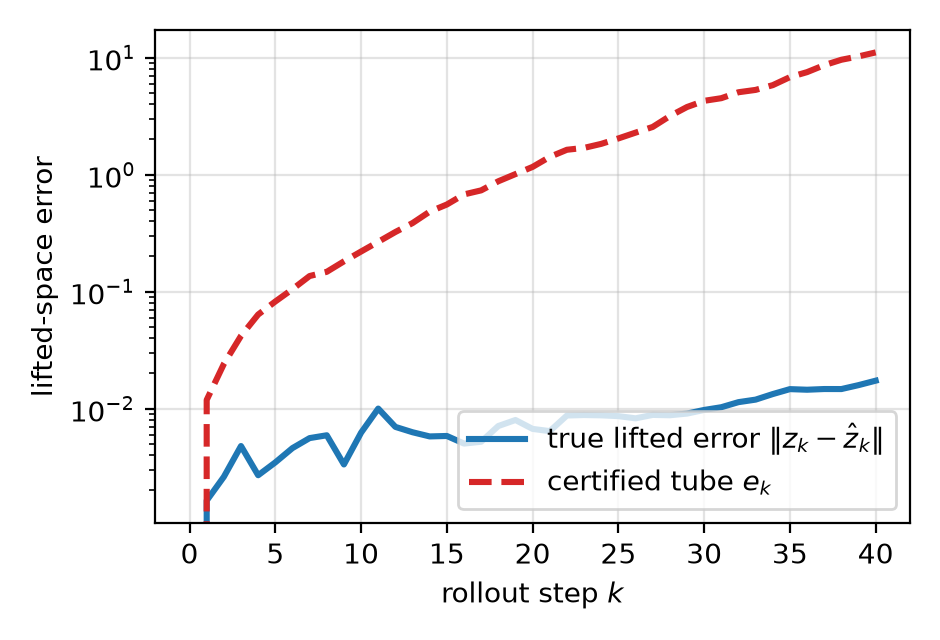
\includegraphics[width=\linewidth]{fig_tube.png}
\caption{Error tube $e_k$ (Prop.~\ref{prop:tube}) vs.\ the true lifted error on a held-out rollout of the \emph{deep bilinear} unicycle model, with $c_x,c_u$ fitted to the model's residuals as an empirical proxy for certified constants. The tube contains the error at every step (zero violations over $82{,}000$ steps), but with $\|A\|_2\!\approx\!1.02$ it is conservative; SafEDMD-grade identification would tighten it.}
\label{fig:tube}
\end{figure}

\subsection{Ablations and design choices}\label{subsec:ablation}
Three choices proved decisive and double as ablations.
\emph{Zero-initialized bilinear terms.}
Initializing $\{B_i\}$ to zero makes training start from the linear model~\eqref{eq:lin} and improve monotonically; random initialization instead yields rollout-unstable models---the failure mode behind a naive bilinear quadrotor, whose four input matrices make an unconstrained fit harder to roll out than the linear one.
\emph{Multi-step training.}
One-step regression of either model gives poor long-horizon rollouts that diverge well before the planning horizon; the $H$-step loss~\eqref{eq:trainloss}, applied identically to both methods, is what makes either model usable inside MPPI.
\emph{The error-tube weight $\beta$.}
Setting $\beta{=}0$ recovers plain bilinear MPPI and is best for nominal regulation, where the surrogate is accurate; $\beta{>}0$ trades a little nominal performance to keep the search inside the certified region, and pays off precisely when the model is least trustworthy---on a weakly identified system or near constraints---consistent with its role as a conservatism knob rather than a performance term.

\begin{table}[t]\centering
\caption{Summary across systems.}
\label{tab:summary}
\begin{tabularx}{\linewidth}{l *{3}{>{\centering\arraybackslash}X}}
\hline
System & Coupling & Ours\,/\,MPPI-DK & Remark\\
\hline
Unicycle  & 1st (heading)  & park $95\%$\,/\,$0\%$ & $37$--$48\times$ pred.\\
7-DOF arm & 1st (Jacobian) & $0.13$\,/\,$0.62$\,m  & linear $0/7$; high var.\\
Pendulum  & weak           & succeed\,/\,succeed   & $4\times$ fewer neurons\\
Quadrotor & 2nd (thrust)   & fly\,/\,fly           & parity\\
\hline
\end{tabularx}
\par\smallskip
{\footnotesize ``Coupling'' is the order at which the input enters the tracked output; ``Ours\,/\,MPPI-DK'' reports parking rate over $20$ trials (unicycle) and mean final error over five seeds (arm). Bilinear is the default; the second-order quadrotor (Sec.~\ref{sec:conclusion}) is the single exception, where a linear lift suffices.}
\end{table}

\subsection{Toward hardware validation}
{\color{red}
\textbf{[Planned --- not yet run.]}
The simulations above isolate the mechanism in a noise-free setting; a hardware study is in preparation to confirm it survives real sensing, actuation, and identification noise.
The primary platform is a differential-drive ground robot, whose forward-speed and yaw-rate commands enter its planar position through the heading---the canonical first-order, configuration-dependent coupling of Prop.~\ref{prop:crit}, and thus the sharpest real-world test of the criterion.
A bilinear and a linear deep Koopman model are identified from the same on-board odometry logs (several minutes of teleoperated and randomized driving) with no analytical model supplied to either controller.
Both controllers then run a goal-reaching and parking task at the platform's native control rate, with pose ground truth from an overhead motion-capture system.
We anticipate the simulation gap to persist on hardware: the bilinear-model controller should park within a few centimetres of the goal across a battery of start--goal pairs, whereas the linear-model controller, unable to represent the heading rotation, should systematically veer off and stall---the closed-loop reflection of the $37$--$48\times$ open-loop prediction gap of Sec.~\ref{sec:exp}.
A second study on a velocity-controlled $6$-DOF manipulator (Jacobian coupling) is planned to reproduce the reach-versus-fail outcome of Fig.~\ref{fig:armbar} on real hardware.
Final measurements, success rates, and videos will be posted to the project page.
}

\begin{figure}[t]\centering
\figph{3.6cm}{\textcolor{red}{Differential-drive ground robot parking under bilinear vs.\ linear Koopman MPPI, with motion-capture ground truth. Hardware photograph and overlaid closed-loop trajectories to be added once the study is run.}}
\caption{\textcolor{red}{[Planned] Real-robot parking. Anticipated outcome: the bilinear-model controller (ours) reaches the goal pose, while the linear-model controller (MPPI-DK) veers off, reproducing the simulation result of Fig.~\ref{fig:unicycle} on hardware.}}
\label{fig:hw}
\end{figure}

%==============================================================
\section{Discussion and Conclusion}\label{sec:conclusion}
%==============================================================
This paper makes a single claim: for sampling-based predictive control of control-affine systems, the bilinear Koopman model is the right default rollout.
Sampling removes the only reason the field has kept the lift linear (the convexity that Koopman MPC requires and MPPI does not), so the provably correct bilinear class costs nothing extra to roll out, and the experiments show that using it rather than a linear surrogate is what separates reaching the goal from structural failure on first-order-coupled robots.
Keeping the lift linear is therefore not a neutral simplification but a forfeiture of the input channel; the accompanying error-tube cost and free-energy guarantee make the bilinear rollout error-aware and practically stable.

\textbf{The boundary of the default.}
The claim is not that bilinearity is universally superior, and a quadrotor marks the precise edge where it is not needed.
When the input reaches the tracked output only at \emph{second} order (thrust drives position through acceleration), the state-dependence of the input map is integrated once more and diluted to $O(\Delta t^2)$, so a constant input matrix is no longer a forfeiture.
The split is visible in prediction (Fig.~\ref{fig:quad}): the bilinear model is $2$--$4\times$ more accurate on the \emph{full} state, capturing the thrust--attitude coupling, yet on the control-relevant \emph{velocity} the two models coincide and both controllers fly to the goal.
Here a linear lift is in fact \emph{preferable}: fewer parameters and an easier fit, with the bilinear model's extra input matrices offering no return and, left untreated, even hurting trainability.
We read this not as a failure mode but as a cleanly closed exemption: the first- versus second-order criterion (Prop.~\ref{prop:crit}, Remark~\ref{rem:order}) tells a practitioner exactly when the linear default is safe, and that corner is narrow and characterizable.

\begin{figure}[t]\centering
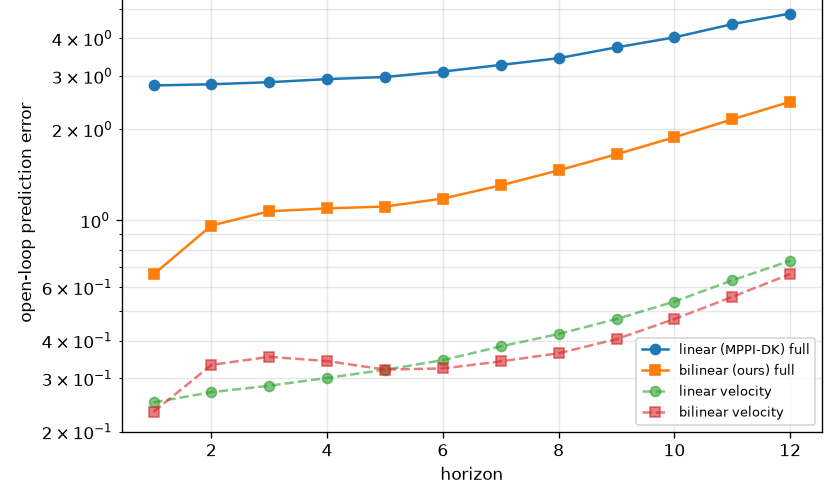
\includegraphics[width=\linewidth]{fig_quad.png}
\caption{The boundary case. Quadrotor open-loop prediction error vs.\ horizon: the bilinear model is $2$--$4\times$ better on the \emph{full} state (it captures the thrust--attitude coupling), but on the control-relevant \emph{velocity} the linear and bilinear curves coincide. Second-order, acceleration-mediated coupling is the delimited regime where a linear lift suffices---indeed is preferable.}
\label{fig:quad}
\end{figure}

\textbf{Relation to prior work and scope.}
The result complements rather than competes with linear Koopman control: linear-predictor Koopman MPC~\cite{korda2018mpc,strasser2026} and MPPI-DK~\cite{mppidk2026} remain well matched to the second-order and weakly coupled regime above, and the contribution here is to lift the linear restriction wherever first-order coupling makes it costly.
The same criterion bounds our own scope: it presumes a tracked output that couples to the input through smooth first-order kinematics, so contact-rich, hybrid dynamics such as legged locomotion, which interleave configuration-dependent coupling with switching contacts that no smooth Koopman lift captures cleanly, are left to future work.

Two limitations remain.
First, optimizing the bilinear model grows harder with the input dimension (Sec.~\ref{sec:exp}): high-DOF lifts train less reliably than the convex linear fit, so closed-loop success, oracle-accurate when achieved, varies across seeds, and stability-constrained identification is the natural remedy.
Second, our stability guarantee presumes a certified error bound that the deep dictionary does not yet furnish, so the fitted constants of Sec.~\ref{sec:exp} stand only as an empirical proxy; supplying genuine certificates through certified (kernel- or SafEDMD-based) identification, which would also yield the small constants a contractive tube requires, together with the hardware studies, are the immediate next steps.
The takeaway is a default with a known boundary: in sampling-based Koopman control, roll out the bilinear model unless the input reaches the tracked output only at second order.

\bibliographystyle{IEEEtran}
\bibliography{IEEEabrv, references, ours}

\end{document}
